\section{Latent Dirichlet Allocation}
\label{sec:topic_modeling_lda}


The assumptions of LDA:
\begin{itemize}
	\item Each topic is a distribution over words.
	\item Each document is a mixture of corpus-wide topics.
	\item Each word is sampled from one of topics. 
\end{itemize}
The LDA attempts to model the document generation process stochastically. However, we have to infer the latent structure (the distributions) of documents. 

\begin{figure}[h]
	\centering
	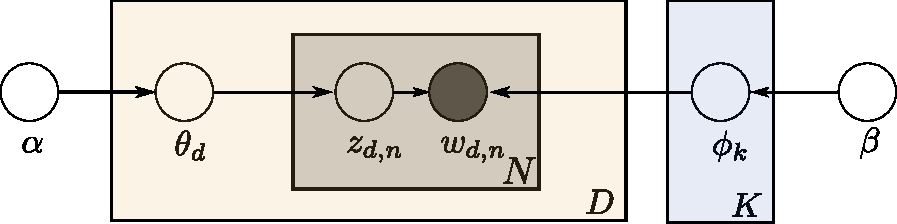
\includegraphics[scale=1.0]{./images/lda/lda.pdf}
\end{figure}
\begin{itemize}
	\item $\theta_d\sim Dir(\alpha)$: For each document, draw topic distribution. 
		\begin{itemize}
			\item $\alpha$: Dirichlet parameter
		\end{itemize}
	\item $z_{d,n}\sim Mult(\theta_d)$: per-word topic assignment. The $n$-th word of document $d$ is from which topic?
	\item $w_{d,n}\sim Mult(\phi_{z_{d,n}},n)$: observed word. The $n$-th word in a document $d$ is from a certain topic ($z_{d,n}$) distribution $\phi_{z_{d,n}}$.
	\item $\phi_k\sim Dir(\beta), i=\{1,\dots,K\}$: topics.
		\begin{itemize}
			\item $\beta$: topic hyperparameter (Dirichlet parameter).
		\end{itemize}
\end{itemize}
The document generation process can be modelled as follows:
\begin{align*}
	p(\phi_{1:K}, \theta_{1:D}, z_{1:D}, w_{1:D}) = \prod_{i=1}^K p(\phi_i|\beta)\prod_{d=1}^D p(\theta_d|\alpha)\bigg(\prod_{n=1}^N p(w_{d,n}|\phi_{1:K},z_{d,n})p(z_{d,n}|\theta_d)\bigg).
\end{align*}

\subsection{LDA Inference}
The posterior of the latent variables given the document is
\begin{align*}
	p(\phi, \theta, \mathbf{z}|\mathbf{w}) = \frac{p(\phi, \theta, \mathbf{z},\mathbf{w})}{\int_{\phi}\int_{\theta}\sum_{\mathbf{z}}p(\phi, \theta, \mathbf{z},\mathbf{w})}
\end{align*}
\begin{itemize}
	\item The denominator is intractable
\end{itemize}
We want to estimate the topic distribution $\mathbf{z}$. 

\subsection{Dirichlet Distribution}
The Dirichlet Distribution can be considered as a extension of the beta distribution. 
\begin{align}
	p(P=\{p_i\}|\alpha_i) = \frac{\Gamma(\sum_i\alpha_i)}{\prod_i\Gamma(\alpha_i)}\prod_ip_i^{\alpha_i-1}
	\label{eq:dirichlet_dist}
\end{align}
\begin{itemize}
	\item $\sum_ip_i = 1$
	\item The posterior distribution of Dirichlet distribution is also Dirichlet distribution. 
\end{itemize}
